%%%%%%%%%%%%%%%%%%%%%%%%%%%%%%%%%%%%%%%%%
% a0poster Landscape Poster
% LaTeX Template
% Version 1.0 (22/06/13)
%
% The a0poster class was created by:
% Gerlinde Kettl and Matthias Weiser (tex@kettl.de)
% 
% This template has been downloaded from:
% http://www.LaTeXTemplates.com
%
% License:
% CC BY-NC-SA 3.0 (http://creativecommons.org/licenses/by-nc-sa/3.0/)
%
%%%%%%%%%%%%%%%%%%%%%%%%%%%%%%%%%%%%%%%%%

%----------------------------------------------------------------------------------------
%	PACKAGES AND OTHER DOCUMENT CONFIGURATIONS
%----------------------------------------------------------------------------------------

\documentclass[a0,landscape]{a0poster}

\usepackage{multicol} % This is so we can have multiple columns of text side-by-side
\columnsep=100pt % This is the amount of white space between the columns in the poster
\columnseprule=3pt % This is the thickness of the black line between the columns in the poster

\usepackage[svgnames]{xcolor} % Specify colors by their 'svgnames', for a full list of all colors available see here: http://www.latextemplates.com/svgnames-colors

%\usepackage{times} % Use the times font
%\usepackage{palatino} % Uncomment to use the Palatino font

\usepackage{graphicx} % Required for including images
\graphicspath{{figures/}} % Location of the graphics files
\usepackage{booktabs} % Top and bottom rules for table
\usepackage[font=small,labelfont=bf]{caption} % Required for specifying captions to tables and figures
\usepackage{amsfonts, amsmath, amsthm, amssymb} % For math fonts, symbols and environments
\usepackage{wrapfig} % Allows wrapping text around tables and figures
% macros.tex
%   Various macros that help with formatting
%   homework assignments and problem sets in LaTeX
%
% James Mason
%

\global\def\TODO{\mathbb{TODO}}
\global\def\median{\mathrm{median}}
\global\def\E{\mathbb{E}}
\global\def\independent{\perp\!\!\!\perp}
\newcommand{\matr}[1]{\mathbf{#1}}


\begin{document}

%----------------------------------------------------------------------------------------
%	POSTER HEADER 
%----------------------------------------------------------------------------------------

% The header is divided into three boxes:
% The first is 55% wide and houses the title, subtitle, names and university/organization
% The second is 25% wide and houses contact information
% The third is 19% wide and houses a logo for your university/organization or a photo of you
% The widths of these boxes can be easily edited to accommodate your content as you see fit

\begin{minipage}[b]{0.53\linewidth}
\Huge{\color{NavyBlue} \scshape An Examination of Tutoring Efficacy in Schools} \\ % Title
\huge\textbf{James Mason \& Nima Hejazi}\\ % Author(s)
\Large{\scshape Ph 242c / Stats 247c --- Longitudinal Data Analysis} \\ % Subtitle
\LARGE{\scshape University of California, Berkeley}\\ % University/organization
\end{minipage}%
%
\colorbox{LightSteelBlue}{\begin{minipage}[b]{0.35\linewidth}
        \vspace{2ex}
        \leftskip 1em \rightskip 1em
        \begin{center}
        {\color{Black} \LARGE \bfseries Research Question}
        \end{center}
          
        \Large
        Does tutoring in reading, provided by the BUILD program,
        to elementary school children in Berkeley public schools,
        have a discernible effect on the reading scores of
        these children, as measured by the TWCRP?
        \vspace{2ex}
\end{minipage}}
\hfill

\includegraphics[scale=0.5]{logo_cal.jpg} 

\vspace{0.5cm} % A bit of extra whitespace between the header and poster content


%----------------------------------------------------------------------------------------

\begin{multicols}{3} % This is how many columns your poster will be broken into, a poster with many figures may benefit from less columns whereas a text-heavy poster benefits from more


%----------------------------------------------------------------------------------------
%	INTRODUCTION
%----------------------------------------------------------------------------------------

\color{SaddleBrown} % SaddleBrown color for the introduction

\section*{Introduction}

BUILD is a tutoring service, offered by CalCorps, that provides after-school 1-to-1 tutoring for students at 11 elementary schools in the Berkeley Unified School District (BUSD). Teachers and literacy coaches at schools identify potential tutees' by reading ability and availability after school. \\

In the year 2014-15, a total of 476 students participated in the BUILD tutoring program. The number of tutoring sessions ranged from 1 to 86, with an average of 15.6. For the evaluation of this program, we have access to the BUSD administrative records, including the district's reading assessments, given 3 times per year, as well as student background information (race/ethnicity, gender, SES, primary language spoken at home) for all K-5 students in Berkeley Unified School District ($N = 4,252$). The data analyzed is for a subset of students, for which the district assessment data and tutoring session information are available for two more years (2012-13, 2013-14).

%----------------------------------------------------------------------------------------
%	MATERIALS AND METHODS
%----------------------------------------------------------------------------------------

\color{NavyBlue}
\section*{Data and Methodology}

%------------------------------------------------

\subsection*{Data}

The data is entirely observational. The treatment -- that is, tutoring -- was not randomly assigned, as a number of factors impacted whether students were able to participate in the program. \\

The data is hierarchical in nature -- that is, there is a nesting structure, with schools ($n=11$) being at the highest level, followed by teachers ($n=201$), and then students ($n=4,252$), with the longitudinal outcome being reading measurements (administered 3 times per year to all students). \\

The longitudinal outcome measure is the Teacher's College Reading \& Writing Project (TCRWP). Scores for each student are transformed via a scaling procedure such that each single point of the examined score represents one year of growth in reading ability. The exam is administered individually to each student in the Fall, Winter, and Spring terms.

\begin{align*}
\text{\textbf{Time-varying}} & \text{ \textbf{variables:}} \\
\mathit{Post}_{ij}: & \text{ The reading score of student } i \text{ at the end of semester } j \\
\mathit{Pre}_{ij}: & \text{ The reading score of student } i \text{ at the start of semester } j \\
\mathit{T}_{ij}: & \text{ Number of tutoring sessions for student } i  \text{ in semester } j \\
\overrightarrow{\mathit{Gr}}_{ij}: & \text{ Vector of dummies for student } i 
      \text{ being in grade } g \text{ in semester } j \\
  & ~ g \in \{\mathrm{K}, 1, 2, 4, 5\} \text {, with 3 as reference}  \\
\\
\text{\textbf{Time-invariant}} & \text{ \textbf{variables:}} \\
\mathit{Post}_{i*}: & \text{ The reading score of student } i \text{ on the most recent test } \\
\mathit{Pre}_{i0}: & \text{ The reading score of student } i \text{ when first enrolled } \\
\mathit{T}_{i*}: & \text{ Total number of tutoring sessions for student } i \\
\mathit{Sem}_{i*}: & \text{ Semesters to date, since enrollment for student } i \\
\mathit{F}_{i}: & \text{ Dummy for student } i  \text{ being female } \\ 
\mathit{En}_{i}: & \text{ Dummy for student } i \text{'s home language being English } \\ 
\mathit{Ed}_{i}: & \text{ Dummy for student } i \text{'s parent having gone to Grad School} \\ 
\mathit{D}_{i}: & \text{ Dummy for student } i \text{ being Socioeconomically Disadvantaged } \\ 
\end{align*}

\subsection*{Methods - Exploratory Analysis}

In order to explore any relationships potentially present in the data, a number of models -- all making use of simple ordinary least squares (OLS) -- were fit. The full model, with an interaction term for treatment and grade, was fit. This model was compared to a main-terms model lacking the covariate race. As a final step, the simplest model, including only post-exam score and pre-exam score, was fit. A comparison revealed the main-terms model had the lowest AIC, with an $R^{2}$ similar to the most complex model. Thus, terms included in this model were chosen for use in the longitudinal analyses fit to analyze the effect of tutoring on reading ability growth.

\subsection*{Methods - Longitudinal Analysis}

\begin{align}
\mathit{Post}_{ij} = & ~ \beta_0 
                     + \beta_1 \mathit{Pre}_{ij}
                     + \beta_2 \mathit{T}_{ij}
                     + \vec\beta_{3} \overrightarrow{\mathit{Gr}}_{ij}
                     + \beta_4 \mathit{F}_{i}
                     + \beta_5 \mathit{En}_{i}
                     + \beta_6 \mathit{Ed}_{i}
                     + \beta_7 \mathit{D}_{i}
                     + \epsilon_{ij}
                     \label{eq:model1} \\
\E(\epsilon_{ij} | \matr{X} ) = & ~ 0 \nonumber \qquad
\mathit{Var}(\epsilon_{ij} | \matr{X} ) = \sigma^2_{\epsilon} \qquad
                    \mathit{Corr}(\epsilon_{ij}, \epsilon_{i'j}) = 0 \qquad
                    \mathit{Corr}(\epsilon_{ij'}, \epsilon_{ij'}) = \rho \nonumber \\
\nonumber \\
\mathit{Post}_{ij} = & ~ \beta_0 + \beta_{0i}
                     + \beta_1 \mathit{Pre}_{ij}
                     + \beta_2 \mathit{T}_{ij}
                     + \vec\beta_{3} \overrightarrow{\mathit{Gr}}_{ij}
                     + \beta_4 \mathit{F}_{i}
                     + \beta_5 \mathit{En}_{i}
                     + \beta_6 \mathit{Ed}_{i}
                     + \beta_7 \mathit{D}_{i}
                     + \epsilon_{ij}
                     \label{eq:model2} \\
\E(\epsilon_{ij} | \matr{X} ) = & ~ 0 \nonumber \qquad
\mathit{Var}(\epsilon_{ij} | \matr{X} ) = \sigma^2_{\epsilon} \qquad
                    \mathit{Corr}(\epsilon_{ij}, \epsilon_{i'j}) = 0 \qquad
                    \mathit{Corr}(\epsilon_{ij'}, \epsilon_{ij'}) = 0 \nonumber \\
\E(\beta_{0i} | \matr{X} ) = & ~ 0 \nonumber \qquad
\mathit{Var}(\beta_{0i} | \matr{X} ) = \sigma^2_{\beta_0} \qquad
                    \mathit{Corr}(\beta_{0i}, \beta_{0i'}) = 0 \nonumber \\
\nonumber \\
\mathit{Post}_{i*} = & ~ \beta_0
                     + \beta_1 \mathit{Pre}_{i0}
                     + \beta_2 \mathit{T}_{i*}
                     + \beta_3 \mathit{Sem}_{i*}
                     + \beta_4 \mathit{F}_{i}
                     + \beta_5 \mathit{En}_{i}
                     + \beta_6 \mathit{Ed}_{i}
                     + \beta_7 \mathit{D}_{i}
                     + \epsilon_{i}
                     \label{eq:model3} \\
\E(\epsilon_{i} | \matr{X} ) = & ~ 0 \nonumber \qquad
\mathit{Var}(\epsilon_{i} | \matr{X} ) = \sigma^2_{\epsilon} \qquad
                    \mathit{Corr}(\epsilon_{i}, \epsilon_{i'}) = 0  \nonumber
\end{align} 

Model~\ref{eq:model1} is a dynamic model, fit using GEE, with an exchangeable correlation structure.
Talk more about the symbols and what they mean.
Explain the coefficient(s) of interest more...

Model~\ref{eq:model2} is a dynamic model with a random intercept.
Talk more about the symbols and what they mean.
Explain the coefficient(s) of interest and the controls.
(Need to report the level-2 variance and/or the ICC in the table
and report discuss it in the results.)

Model~\ref{eq:model3} is a cross-sectional model, where the
entire history of the student has been collapsed into a
single observation.  Explain the new covariates.
Talk more about the symbols and what they mean.
Explain the coefficient(s) of interest and the controls.



%----------------------------------------------------------------------------------------
%	RESULTS 
%----------------------------------------------------------------------------------------

\color{NavyBlue}

\section*{Results}

%
\color{Black}
\begin{center}\vspace{1cm}
{
\def\sym#1{\ifmmode^{#1}\else\(^{#1}\)\fi}
\begin{tabular}{l*{3}{cc}}
\toprule
                    &\multicolumn{2}{c}{(1)}           &\multicolumn{2}{c}{(2)}           &\multicolumn{2}{c}{(3)}           \\
                    &\multicolumn{2}{c}{Dynamic (GEE)} &\multicolumn{2}{c}{Dynamic (RI)}  &\multicolumn{2}{c}{Cross-sectional}\\
\midrule
Test Score at Start of Semester&        0.89\sym{***}&      (0.03)&        0.87\sym{***}&      (0.04)&                     &            \\
Test Score at Initial Enrollment&                     &            &                     &            &        0.89\sym{***}&      (0.07)\\
\# Sessions per Semester&        0.00         &      (0.00)&        0.00         &      (0.00)&                     &            \\
\# Sessions Total   &                     &            &                     &            &       -0.01\sym{*}  &      (0.00)\\
\# Semesters Since Enrollment&                     &            &                     &            &        0.55\sym{***}&      (0.03)\\
Grade Level \\ \qquad K                   &       -0.20\sym{*}  &      (0.10)&       -0.24\sym{*}  &      (0.11)&                     &            \\
\qquad 1                   &       -0.07         &      (0.06)&       -0.10         &      (0.07)&                     &            \\
\qquad 2                   &       -0.04         &      (0.03)&       -0.05         &      (0.03)&                     &            \\
\qquad 3            &        ref.         &            &        ref.         &            &                     &            \\
\qquad 4                   &        0.12\sym{**} &      (0.04)&        0.12\sym{**} &      (0.04)&                     &            \\
\qquad 5                   &        0.37\sym{***}&      (0.07)&        0.40\sym{***}&      (0.08)&                     &            \\
Female              &        0.00         &      (0.02)&        0.00         &      (0.02)&        0.25\sym{*}  &      (0.12)\\
Native English Speaker&       -0.01         &      (0.02)&       -0.01         &      (0.02)&       -0.04         &      (0.13)\\
Parent Went to Grad School&        0.05\sym{*}  &      (0.02)&        0.06\sym{*}  &      (0.02)&        0.34\sym{*}  &      (0.16)\\
Socioeconomically Disadvantaged&       -0.00         &      (0.02)&       -0.00         &      (0.02)&       -0.01         &      (0.16)\\
(Intercept)         &        0.58\sym{***}&      (0.07)&        0.62\sym{***}&      (0.08)&       -0.20         &      (0.26)\\
\midrule
Observations        &        1153         &            &        1153         &            &         128         &            \\
Groups              &         541         &            &         541         &            &                     &            \\
$\rho$              &                     &            &       0.057         &            &                     &            \\
\bottomrule
\multicolumn{7}{l}{\footnotesize Robust standard errors in parentheses}\\
\multicolumn{7}{l}{\footnotesize \sym{*} \(p<0.05\), \sym{**} \(p<0.01\), \sym{***} \(p<0.001\)}\\
\end{tabular}
}

\captionof{table}{\color{Green} Estimates, Standard Errors, and Significance for the three longitudinal models examined.}
\end{center}\vspace{1cm}
\color{NavyBlue}
%   

In all cases, the longitudinal models fit reveal that the best predictor of post-exam score is the most recent pre-exam score, for a given term. While differences in reading ability were predicted by grade level, this effect is most easily interpreted as differences in reading ability development of children; this is corroborated by the significance of the estimated coefficient for the number of semesters since student enrollment. In regard to our question of interest, it was found that the number of tutoring sessions (and the number of semesters a student received tutoring) had a (slightly) negative effect on student performance, interpreted as falling behind in reading ability. 

\color{NavyBlue}

\begin{center}\vspace{1cm}
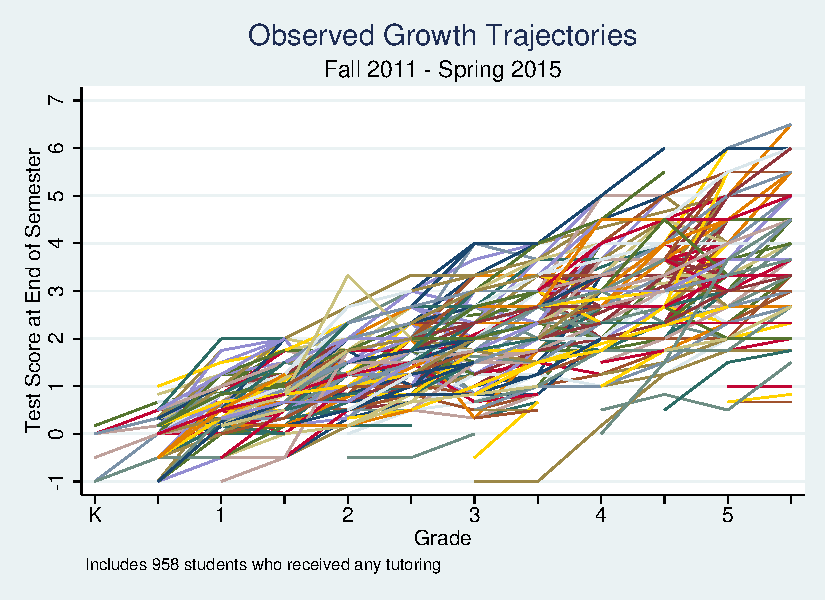
\includegraphics[width=0.8\linewidth]{xtline.pdf}
\captionof{figure}{\color{Green} Student Growth Trajectories}
\end{center}\vspace{0.5cm}

The trajectory plot illustrates the growth of students over time as assessed by the TCRWP scores administered several times per academic year. As expected, the performance of students increases over time, though modeling reveals that tutoring is unlikely to be the cause of this growth.

%----------------------------------------------------------------------------------------
%	CONCLUSIONS
%----------------------------------------------------------------------------------------

\color{SaddleBrown} % SaddleBrown color for the conclusions to make them stand out

\section*{Conclusions and Further Considerations}

\begin{itemize}
\item All of the analyses, including the GEE, random intercept, and cross-sectional history models, show that tutoring is not effective in improving reading scores, while the best predictor of the post-exam score -- in any term -- is the pre-exam score (the score from the previous term).
\item The observed data structure is quite complicated, as illustrated by the causal DAG below. There are limitations to the methods discussed; in future work, care ought to be taken to account for the causal relationships between the covariates, treatment, and outcome in the investigations.
\end{itemize}

\color{DarkSlateGray} % Set the color back to DarkSlateGray for the rest of the content

\begin{center}\vspace{1cm}
<<<<<<< HEAD
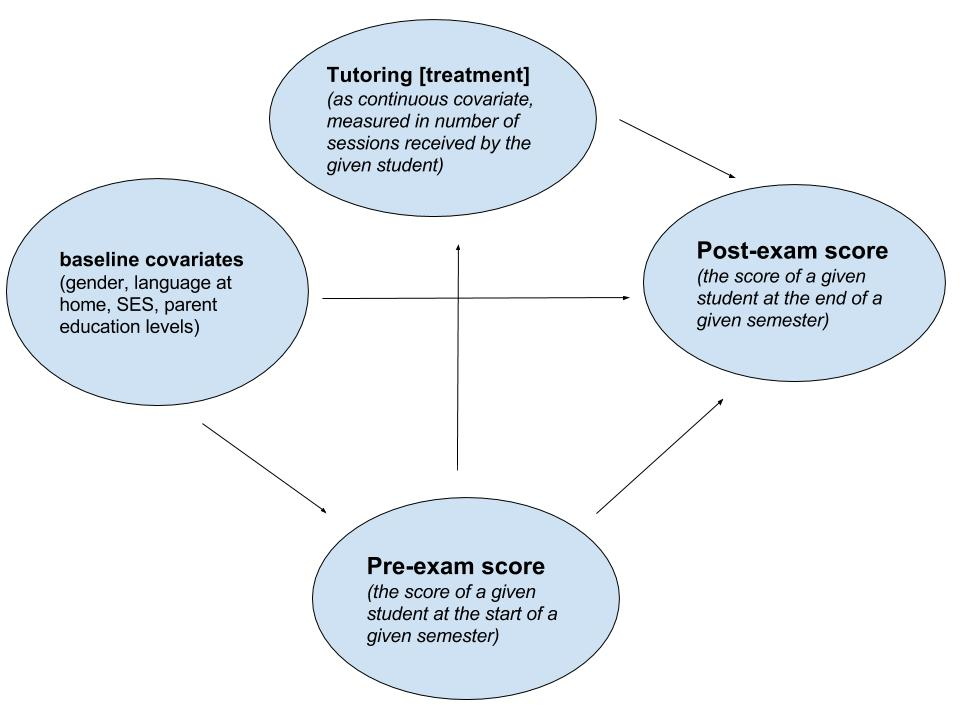
\includegraphics[width=0.8\linewidth]{LongitData-DAG.jpg}
\captionof{figure}{\color{Green} Descriptive directed acyclic graph (DAG) of the causal relationships present in the observed data structure.}
\end{center}\vspace{-1cm}
=======
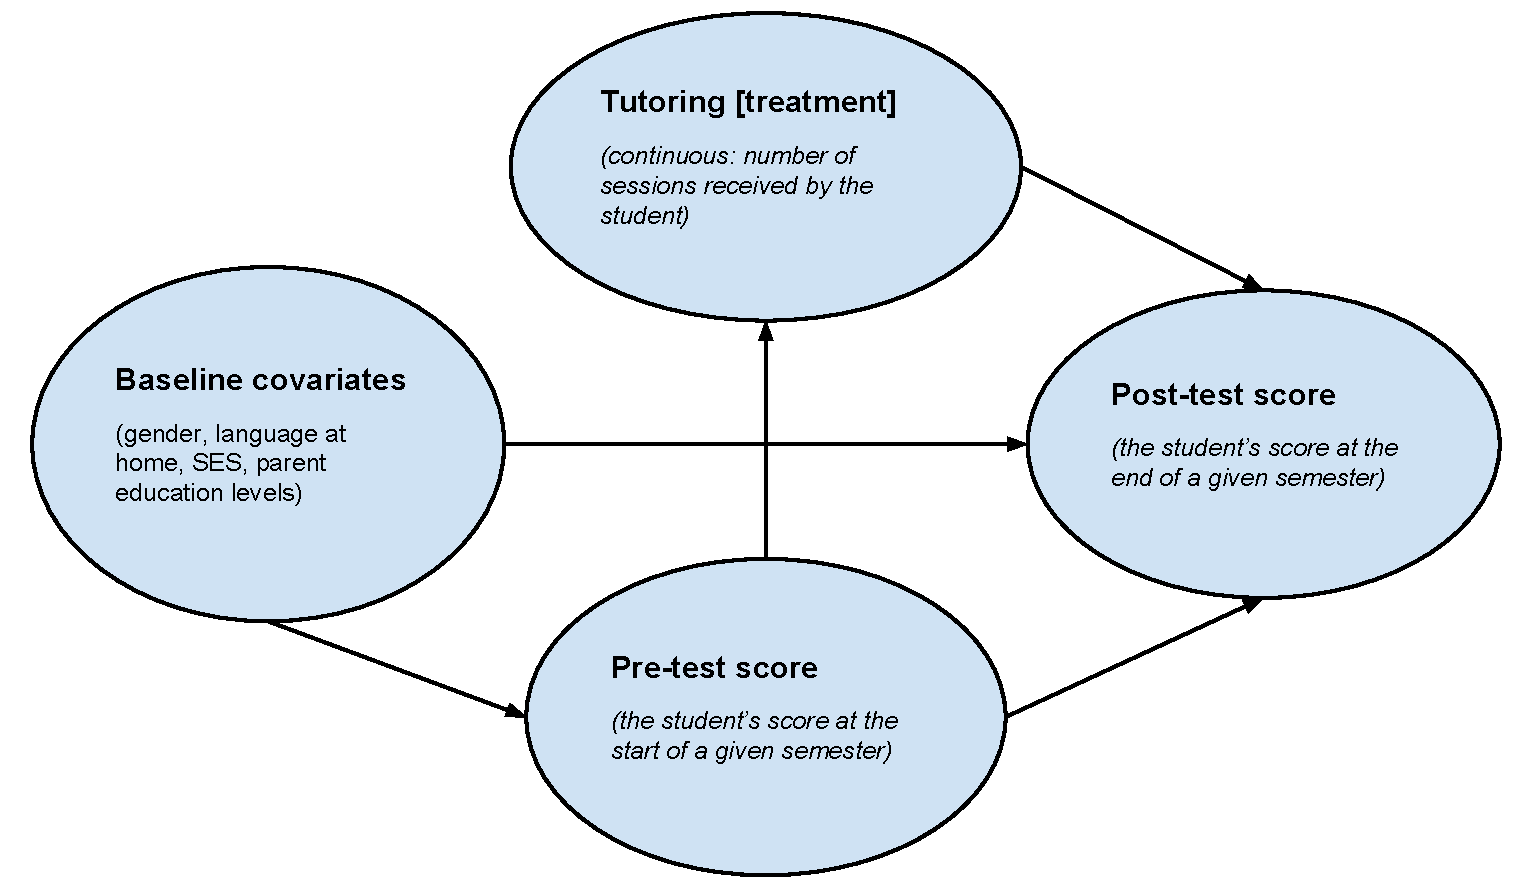
\includegraphics[width=0.8\linewidth]{LongitData-DAG.pdf}
\captionof{figure}{\color{Green} Causal DAG}
\end{center}\vspace{1cm}
>>>>>>> 9d7400f6e0bd41a1bb233c5536bfe94444f9536e

%----------------------------------------------------------------------------------------
%	ACKNOWLEDGEMENTS
%----------------------------------------------------------------------------------------

\section*{Acknowledgements}

Yukie Toyama, for providing guidance about the BUILD study and her work with the data set.

%----------------------------------------------------------------------------------------

\end{multicols}
\end{document}